\documentclass[12pt,a4paper]{article}
\usepackage[utf8]{vietnam}
\usepackage{amsmath,amssymb,mathrsfs}
\usepackage{graphicx}
\usepackage{tikz}
\usepackage{array}
\usepackage[top=1.4cm,bottom=1.5cm,left=1.6cm,right=1.5cm]{geometry}
\usepackage{fancyhdr}
\usepackage{tcolorbox}
\tcbuselibrary{skins}
\usepackage[dethi]{ex_test}

\makeatletter
\@ifundefined{c@bt}{\newcounter{bt}}{}
\makeatother

\pagestyle{fancy}
\fancyhf{}
\renewcommand{\headrulewidth}{0pt}
\renewcommand{\footrulewidth}{0.4pt}
\lfoot{\footnotesize\textsl{Lớp Toán Cô Thúy -- SĐT: 0935.322.328 -- 50/2C Phạm Thị Liên}}
\rfoot{\footnotesize\textsl{Trang \thepage/4 -- Mã đề 0103}}

\begin{document}

% KHUNG TIÊU ĐỀ CHUẨN TỐI ƯU LỚP TOÁN CÔ THÚY
\noindent
\begin{tabular}{|p{6.6cm}|p{6.4cm}|>{\centering\arraybackslash}p{3.2cm}|}
\hline
\begin{minipage}{6.6cm}
\vspace{5pt}
\centering
{\large\bfseries\color{blue!80!black} LỚP TOÁN CÔ THÚY}\\[4pt]
\textbf{SĐT:} 0935.322.328\\[3pt]
\textbf{Địa chỉ:} 50/2C Phạm Thị Liên
\vspace{5pt}
\end{minipage}
&
\multicolumn{2}{p{10.0cm}|}{
\begin{minipage}{10.0cm}
\vspace{5pt}
\centering
{\bfseries\color{red!80!black} ĐỀ KHẢO SÁT CHẤT LƯỢNG TOÁN 12}\\[4pt]
\textbf{THPT Số 3 Bảo Thắng (2026 -- 2027)}\\[3pt]
\textit{Thời gian làm bài: 25 phút}
\vspace{5pt}
\end{minipage}
} \\
\hline
\rule{0pt}{15pt}Họ và tên: \dotfill\rule[-5pt]{0pt}{5pt} &
\rule{0pt}{15pt}Số báo danh: \dotfill\rule[-5pt]{0pt}{5pt} &
\rule{0pt}{15pt}\textbf{Mã đề 0103}\rule[-5pt]{0pt}{5pt} \\
\hline
\end{tabular}
\vspace{0.2cm}

\begin{flushleft}
	{\color{blue!50!green}\fbox{\fontfamily{qag}\bfseries\selectfont PHẦN I. Câu trắc nghiệm nhiều phương án lựa chọn}}
	\textit{\small (Thí sinh trả lời từ câu 1 đến câu 12. Mỗi câu hỏi thí sinh chỉ chọn một phương án.)}
\end{flushleft}
\setcounter{ex}{0}
\setcounter{bt}{0}

% Câu 1
\begin{ex}
	\immini{
		Cho hàm số bậc ba $y = f(x)$ có đồ thị như hình bên. Hàm số nghịch biến trên khoảng nào sau đây?
		\choice
		{$(-\infty; -1)$}
		{$(1; +\infty)$}
		{\True $(-1; 1)$}
		{$(-\infty; 1)$}
	}{
		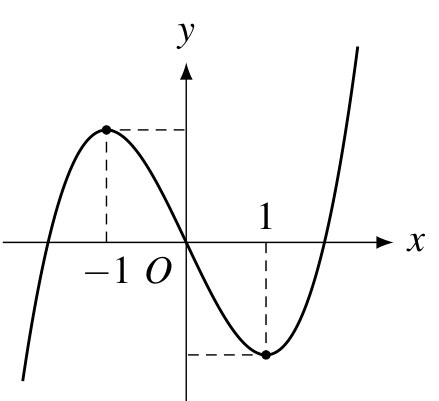
\includegraphics[width=4.2cm]{c1_hinh.png}
	}
	\loigiai{}
\end{ex}

% Câu 2
\begin{ex}
	Cho hàm số $y = f(x)$ có bảng biến thiên như dưới đây:
	\begin{center}
	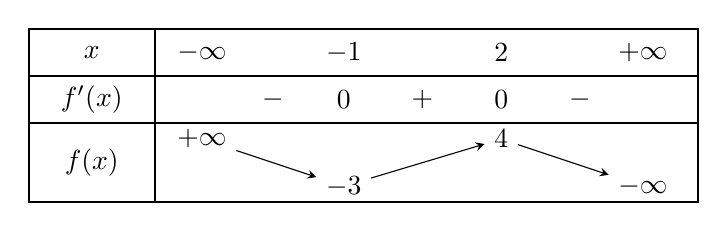
\begin{tikzpicture}[>=stealth,scale=1]
	  \draw[thick] (0,0) rectangle (8.5,-2.2);
	  \draw[thick] (0,-0.6) -- (8.5,-0.6);
	  \draw[thick] (0,-1.2) -- (8.5,-1.2);
	  \draw[thick] (1.6,0) -- (1.6,-2.2);
	  \node at (0.8,-0.3) {$x$};
	  \node at (0.8,-0.9) {$f'(x)$};
	  \node at (0.8,-1.7) {$f(x)$};
	  \node at (2.2,-0.3) {$-\infty$};
	  \node at (4.0,-0.3) {$-1$};
	  \node at (6.0,-0.3) {$2$};
	  \node at (7.8,-0.3) {$+\infty$};
	  \node at (3.1,-0.9) {$-$};
	  \node at (4.0,-0.9) {$0$};
	  \node at (5.0,-0.9) {$+$};
	  \node at (6.0,-0.9) {$0$};
	  \node at (7.0,-0.9) {$-$};
	  \node (p1) at (2.2,-1.4) {$+\infty$};
	  \node (p2) at (4.0,-2.0) {$-3$};
	  \node (p3) at (6.0,-1.4) {$4$};
	  \node (p4) at (7.8,-2.0) {$-\infty$};
	  \draw[->] (p1) -- (p2);
	  \draw[->] (p2) -- (p3);
	  \draw[->] (p3) -- (p4);
	\end{tikzpicture}
	\end{center}
	Giá trị cực tiểu của hàm số là
	\choice
	{\True $-3$}
	{$-1$}
	{$2$}
	{$4$}
	\loigiai{}
\end{ex}

% Câu 3
\begin{ex}
	Cho hàm số $y = \dfrac{x - 4}{2x + 1}$. Tâm đối xứng của đồ thị là
	\choice
	{$I\left(-\dfrac{1}{2}; -\dfrac{1}{2}\right)$}
	{$I\left(\dfrac{1}{2}; -\dfrac{1}{2}\right)$}
	{$I(2; 1)$}
	{\True $I\left(-\dfrac{1}{2}; \dfrac{1}{2}\right)$}
	\loigiai{}
\end{ex}

% Câu 4
\begin{ex}
	Cho hàm số $y = \dfrac{2x + 5}{x + 1}$. Khẳng định nào sau đây đúng?
	\choice
	{Hàm số đồng biến trên từng khoảng xác định}
	{\True Hàm số nghịch biến trên từng khoảng xác định}
	{Hàm số có một điểm cực trị}
	{Đồ thị không có tiệm cận ngang}
	\loigiai{}
\end{ex}

% Câu 5
\begin{ex}
	Cho hàm số $y = x + \dfrac{1}{x}$. Phương trình đường tiệm cận xiên của đồ thị hàm số là
	\choice
	{\True $y = x$}
	{$y = x + 1$}
	{$y = x - 1$}
	{$x = 0$}
	\loigiai{}
\end{ex}

% Câu 6
\begin{ex}
	Cho hàm số $y = x + 1 + \dfrac{2}{x + 1}$. Giao điểm hai đường tiệm cận của đồ thị hàm số là
	\choice
	{$I(1; 2)$}
	{$I(-1; 1)$}
	{\True $I(-1; 0)$}
	{$I(0; -1)$}
	\loigiai{}
\end{ex}

\newpage
% Câu 7
\begin{ex}
	Cho hàm số $y = f(x)$ có đạo hàm $f'(x) = 3(x - 1)(x + 3)$ với mọi $x \in \mathbb{R}$. Điểm cực đại của hàm số đã cho là
	\choice
	{$x = 1$}
	{\True $x = -3$}
	{$x = 3$}
	{$x = -1$}
	\loigiai{}
\end{ex}

% Câu 8
\begin{ex}
	Cho hàm số $y = f(x) = x^3 + 6x^2 + 9x$. Tâm đối xứng của đồ thị là
	\choice
	{$I(-1; 0)$}
	{$I(2; -2)$}
	{$I(-2; 0)$}
	{\True $I(-2; -2)$}
	\loigiai{}
\end{ex}

% Câu 9
\begin{ex}
	Cho hàm số $y = f(x)$ có đạo hàm $f'(x) = x(x - 1)(x + 2)$ với mọi $x \in \mathbb{R}$. Số khoảng đồng biến của hàm số là
	\choice
	{$1$}
	{$3$}
	{\True $2$}
	{$4$}
	\loigiai{}
\end{ex}

% Câu 10
\begin{ex}
	Cho hàm số $y = \dfrac{ax^2 + bx + c}{dx + e}$ ($ad \ne 0$), trong đó đa thức tử không chia hết cho đa thức mẫu. Bảng biến thiên của hàm số được cho như dưới đây:
	\begin{center}
	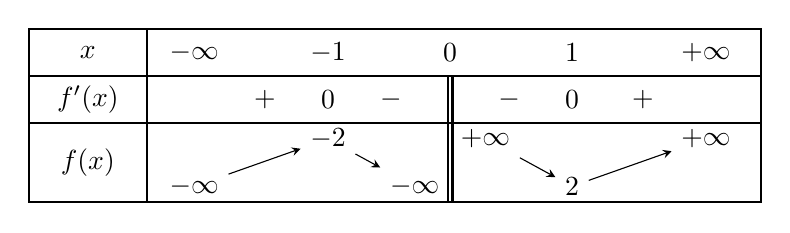
\begin{tikzpicture}[>=stealth,scale=1]
	  \draw[thick] (0,0) rectangle (9.3,-2.2);
	  \draw[thick] (0,-0.6) -- (9.3,-0.6);
	  \draw[thick] (0,-1.2) -- (9.3,-1.2);
	  \draw[thick] (1.5,0) -- (1.5,-2.2);
	  \draw[thick] (5.32,-0.6) -- (5.32,-2.2);
	  \draw[thick] (5.38,-0.6) -- (5.38,-2.2);
	  \node at (0.75,-0.3) {$x$};
	  \node at (0.75,-0.9) {$f'(x)$};
	  \node at (0.75,-1.7) {$f(x)$};
	  \node at (2.1,-0.3) {$-\infty$};
	  \node at (3.8,-0.3) {$-1$};
	  \node at (5.35,-0.3) {$0$};
	  \node at (6.9,-0.3) {$1$};
	  \node at (8.6,-0.3) {$+\infty$};
	  \node at (3.0,-0.9) {$+$};
	  \node at (3.8,-0.9) {$0$};
	  \node at (4.6,-0.9) {$-$};
	  \node at (6.1,-0.9) {$-$};
	  \node at (6.9,-0.9) {$0$};
	  \node at (7.8,-0.9) {$+$};
	  \node (p1) at (2.1,-2.0) {$-\infty$};
	  \node (p2) at (3.8,-1.4) {$-2$};
	  \node (p3) at (4.9,-2.0) {$-\infty$};
	  \node (p4) at (5.8,-1.4) {$+\infty$};
	  \node (p5) at (6.9,-2.0) {$2$};
	  \node (p6) at (8.6,-1.4) {$+\infty$};
	  \draw[->] (p1) -- (p2);
	  \draw[->] (p2) -- (p3);
	  \draw[->] (p4) -- (p5);
	  \draw[->] (p5) -- (p6);
	\end{tikzpicture}
	\end{center}
	Hàm số nào dưới đây có bảng biến thiên đã cho?
	\choice
	{\True $y = \dfrac{x^2 + 1}{x}$}
	{$y = \dfrac{x^2 - 1}{x}$}
	{$y = \dfrac{x^2 + 1}{x - 1}$}
	{$y = \dfrac{x^2 + 4}{x}$}
	\loigiai{}
\end{ex}

% Câu 11
\begin{ex}
	Cho hàm số $y = x + 2 + \dfrac{3}{x - 2}$. Phương trình đường tiệm cận xiên của đồ thị hàm số là
	\choice
	{$x = 2$}
	{$y = 2$}
	{\True $y = x + 2$}
	{$y = x - 2$}
	\loigiai{}
\end{ex}

% Câu 12
\begin{ex}
	Cho hàm số $y = f(x)$ xác định trên $\mathbb{R} \setminus \{-1\}$ và có đạo hàm $f'(x) = \dfrac{x(x + 2)}{(x + 1)^2}$. Điểm cực đại của hàm số đã cho là
	\choice
	{$x = -1$}
	{$x = 0$}
	{$x = 2$}
	{\True $x = -2$}
	\loigiai{}
\end{ex}

\newpage
\begin{flushleft}
	{\color{blue!50!green}\fbox{\fontfamily{qag}\bfseries\selectfont PHẦN II. Câu trắc nghiệm đúng sai}}
	\textit{\small (Thí sinh trả lời từ câu 1 đến câu 4. Trong mỗi ý a), b), c), d) ở mỗi câu, thí sinh chọn đúng hoặc sai.)}
\end{flushleft}
\setcounter{ex}{0}
\setcounter{bt}{0}

% Phần II Câu 1
\begin{ex}
	\immini{
		Cho hàm số $y = \dfrac{2x + 1}{x - 1}$. Xét tính đúng, sai của các phát biểu sau:
		\choiceTF
		{\True Đạo hàm của hàm số là $y' = -\dfrac{3}{(x - 1)^2}$}
		{Hàm số đồng biến trên khoảng $(1; +\infty)$}
		{\True Đồ thị có tiệm cận ngang $y = 2$}
		{Hình bên là đồ thị của hàm số đã cho}
	}{
		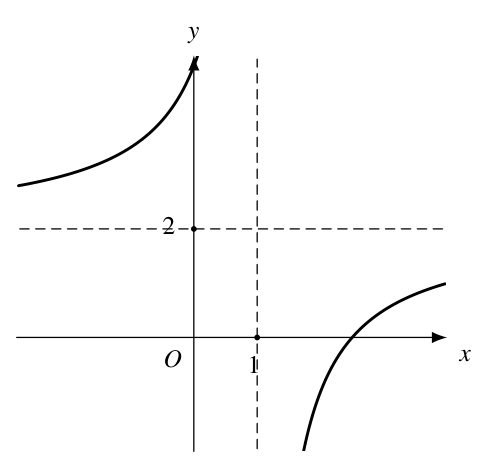
\includegraphics[width=4.2cm]{p2_c1_hinh.png}
	}
	\loigiai{}
\end{ex}

% Phần II Câu 2
\begin{ex}
	\immini{
		Cho hàm số $y = \dfrac{ax^2 + bx + c}{dx + e}$ ($ad \ne 0$), trong đó đa thức tử không chia hết cho đa thức mẫu. Đồ thị của hàm số được cho như hình bên. Xét tính đúng, sai của các phát biểu sau:
		\choiceTF
		{\True Đồ thị có tiệm cận đứng $x = 1$}
		{\True Đường tiệm cận xiên có phương trình $y = x + 2$}
		{Đồ thị cắt trục tung tại điểm có tung độ bằng $2$}
		{Hàm số nghịch biến trên toàn bộ $\mathbb{R}$}
	}{
		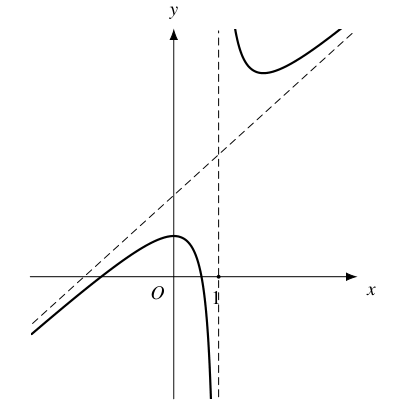
\includegraphics[width=4.0cm]{p2_c2_hinh.png}
	}
	\loigiai{}
\end{ex}

% Phần II Câu 3
\begin{ex}
	Cho hàm số $y = \dfrac{(x - 2)^2}{x - 1}$. Xét tính đúng, sai của các phát biểu sau:
	\choiceTF
	{\True Tập xác định của hàm số là $\mathbb{R} \setminus \{1\}$}
	{Hàm số nghịch biến trên khoảng $(-\infty; 0)$}
	{Hàm số đạt cực tiểu tại $x = 0$}
	{\True Đồ thị có tiệm cận xiên $y = x - 3$}
	\loigiai{}
\end{ex}

% Phần II Câu 4
\begin{ex}
	Cho hàm số $y = f(x) = -x^3 + 3x + 1$. Xét tính đúng, sai của các phát biểu sau:
	\choiceTF
	{\True Đạo hàm của hàm số là $f'(x) = 3(1 - x^2)$}
	{\True Hàm số đồng biến trên khoảng $(-1; 1)$}
	{Giá trị cực tiểu của hàm số bằng $1$}
	{\True Bảng biến thiên dưới đây là bảng biến thiên của hàm số đã cho
		\begin{center}
		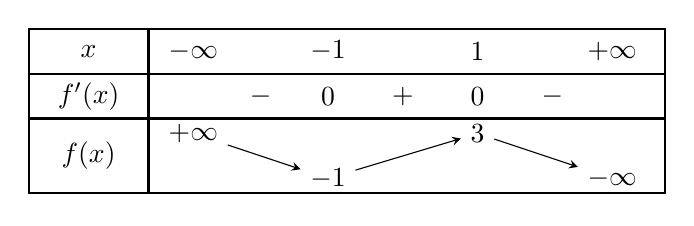
\begin{tikzpicture}[>=stealth,scale=0.95]
		  \draw[thick] (0,0) rectangle (8.5,-2.2);
		  \draw[thick] (0,-0.6) -- (8.5,-0.6);
		  \draw[thick] (0,-1.2) -- (8.5,-1.2);
		  \draw[thick] (1.6,0) -- (1.6,-2.2);
		  \node at (0.8,-0.3) {$x$};
		  \node at (0.8,-0.9) {$f'(x)$};
		  \node at (0.8,-1.7) {$f(x)$};
		  \node at (2.2,-0.3) {$-\infty$};
		  \node at (4.0,-0.3) {$-1$};
		  \node at (6.0,-0.3) {$1$};
		  \node at (7.8,-0.3) {$+\infty$};
		  \node at (3.1,-0.9) {$-$};
		  \node at (4.0,-0.9) {$0$};
		  \node at (5.0,-0.9) {$+$};
		  \node at (6.0,-0.9) {$0$};
		  \node at (7.0,-0.9) {$-$};
		  \node (p1) at (2.2,-1.4) {$+\infty$};
		  \node (p2) at (4.0,-2.0) {$-1$};
		  \node (p3) at (6.0,-1.4) {$3$};
		  \node (p4) at (7.8,-2.0) {$-\infty$};
		  \draw[->] (p1) -- (p2);
		  \draw[->] (p2) -- (p3);
		  \draw[->] (p3) -- (p4);
		\end{tikzpicture}
		\end{center}
	}
	\loigiai{}
\end{ex}

\newpage
\begin{flushleft}
	{\color{blue!50!green}\fbox{\fontfamily{qag}\bfseries\selectfont PHẦN III. Câu trắc nghiệm yêu cầu trả lời ngắn}}
	\textit{\small (Thí sinh trả lời từ câu 1 đến câu 6.)}
\end{flushleft}
\setcounter{ex}{0}
\setcounter{bt}{0}

% Phần III Câu 1
\begin{ex}
	Cho hàm số $y = f(x)$ có bảng biến thiên như dưới đây:
	\begin{center}
	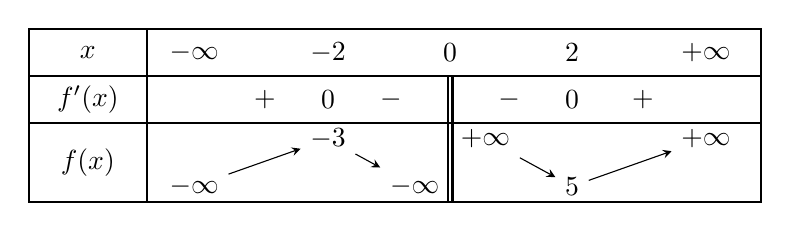
\begin{tikzpicture}[>=stealth,scale=1]
	  \draw[thick] (0,0) rectangle (9.3,-2.2);
	  \draw[thick] (0,-0.6) -- (9.3,-0.6);
	  \draw[thick] (0,-1.2) -- (9.3,-1.2);
	  \draw[thick] (1.5,0) -- (1.5,-2.2);
	  \draw[thick] (5.32,-0.6) -- (5.32,-2.2);
	  \draw[thick] (5.38,-0.6) -- (5.38,-2.2);
	  \node at (0.75,-0.3) {$x$};
	  \node at (0.75,-0.9) {$f'(x)$};
	  \node at (0.75,-1.7) {$f(x)$};
	  \node at (2.1,-0.3) {$-\infty$};
	  \node at (3.8,-0.3) {$-2$};
	  \node at (5.35,-0.3) {$0$};
	  \node at (6.9,-0.3) {$2$};
	  \node at (8.6,-0.3) {$+\infty$};
	  \node at (3.0,-0.9) {$+$};
	  \node at (3.8,-0.9) {$0$};
	  \node at (4.6,-0.9) {$-$};
	  \node at (6.1,-0.9) {$-$};
	  \node at (6.9,-0.9) {$0$};
	  \node at (7.8,-0.9) {$+$};
	  \node (p1) at (2.1,-2.0) {$-\infty$};
	  \node (p2) at (3.8,-1.4) {$-3$};
	  \node (p3) at (4.9,-2.0) {$-\infty$};
	  \node (p4) at (5.8,-1.4) {$+\infty$};
	  \node (p5) at (6.9,-2.0) {$5$};
	  \node (p6) at (8.6,-1.4) {$+\infty$};
	  \draw[->] (p1) -- (p2);
	  \draw[->] (p2) -- (p3);
	  \draw[->] (p4) -- (p5);
	  \draw[->] (p5) -- (p6);
	\end{tikzpicture}
	\end{center}
	Hàm số có bao nhiêu điểm cực trị?
	\par\shortans[oly]{2}
	\loigiai{}
\end{ex}

% Phần III Câu 2
\begin{ex}
	Cho hàm số $y = f(x) = x^3 - 6x^2 + 9x + 1$. Tính hiệu giữa giá trị cực đại và giá trị cực tiểu của hàm số.
	\par\shortans[oly]{4}
	\loigiai{}
\end{ex}

% Phần III Câu 3
\begin{ex}
	Cho hàm số $y = \dfrac{2x + 1}{x - 1}$. Gọi $I(a; b)$ là giao điểm hai đường tiệm cận. Tính $a + b$.
	\par\shortans[oly]{3}
	\loigiai{}
\end{ex}

% Phần III Câu 4
\begin{ex}
	Cho hàm số $y = \dfrac{x^2 - 1}{x - 2}$. Tính tung độ giao điểm của đường tiệm cận xiên của đồ thị với trục tung.
	\par\shortans[oly]{2}
	\loigiai{}
\end{ex}

% Phần III Câu 5
\begin{ex}
	Cho hàm số $y = f(x)$ có đạo hàm $f'(x) = (x + 3)(x - 1)^2(x - 2)$ với mọi $x \in \mathbb{R}$. Tính tổng các giá trị của $x$ tại đó hàm số đạt cực trị.
	\par\shortans[oly]{-1}
	\loigiai{}
\end{ex}

% Phần III Câu 6
\begin{ex}
	Cho hàm số $y = f(x) = x^3 - 3ax$, với $a > 0$. Biết hàm số đạt cực tiểu tại $x = 3$. Tính $a$.
	\par\shortans[oly]{9}
	\loigiai{}
\end{ex}

\vspace{0.4cm}
\begin{center}
	\textbf{------ HẾT ------}
\end{center}

\end{document}
